%!TEX root = ./../thesis.tex

\chapter{Background}
\label{c:background}
This section provides the necessary background to follow the argumentation in the following chapters regarding state centric programming model and consistency management.
This includes an understanding of algorithms and optimization techniques commonly used in practice (not limited to distributed machine learning), the current state-of-the-art in dataflow systems and how dataflow is used to provide a fault tolerant and distributed framework for large scale data processing and machine learning.
Furthermore the field of distributed machine learning is explained in more detail, including the current state-of-the-art frameworks used for this purpose, their limitations and challenges that arise when machine learning algorithms are parallelized in a distributed fashion among multiple physical machines.


\section{Algorithms and Optimization}

\subsection{Iterative Convergent Algorithms}
\label{ss:ica}
Consider a supervised learning setup with a dataset $D = \{z_1,\ldots,z_n\}$ with each example $z_i$ being represented by a pair $(x_i,y_i)$ consisting of an input $x_i$ and a scalar output $y_i$.
Consider also a loss function $\ell(\hat{y},y)$ quantifying the cost of predicting $\hat{y}$ when the true output is $y$. As a model, a family $F$ of functions $f_w(x)$ parameterized by a weight vector $w$ is chosen.
The goal is to find a function $f \in F$ that minimizes the loss $Q(z, w) = \ell(f_w(x),y)$. Emperical risk $E_n(f) = \frac{1}{n}\sum_{i=0}^{n}\ell(f(x_i),y_i)$ performance on training set, expected risk generalization performance.
\begin{equation}
E_n(f_w) = \frac{1}{n}\sum_{i=0}^{n} \ell(f_w(x_i),y_i)
\label{eqn:emp_risk}
\end{equation}
In order to find an optimal solution many algorithms used in large scale machine learning such as regression, topic models, matrix factorization or neural networks employ either gradient based methods or markov chain monte carlo methods.
To obtain the optimal solution those algorithms try to iteratively update the weight vector $w$. At each iteration $t$ an updated weight vector $w^{t}$ is computed based on the vector of the previous iteration $w^{(t-1)}$ and the data $D$. The resulting model $f_{w^{t}}$ is again a better summary of the data $D$ under the objective $Q$. \ref{eqn:delta_upd} shows the process of refining the model, with $\Delta$ being an arbitrary update function.
\begin{equation}
w^{t} = w^{(t-1)} + \Delta(w^{(t-1)},D)
\label{eqn:delta_upd}
\end{equation}
The update function depends on the algorithm employed and can be viewed as a procedure of obtaining a step towards a better model. At each iteration an update $\Delta w$ is computed and applied to the previous weight vector until a stopping condition is satisfied. E.g. the distance to the optimal solution or the objective difference between two iterations is monitored. When the difference is below a certain threshold the computation stops and the algorithm is said to be converged.


\subsection{Convex Optimization}
\label{ss:optimization}
In order to estimate the optimal parameters $w^*$ of a function belonging to class $f_{w^*} \in F$, numerous techniques can be employed to estimate said parameters.
In many cases, especially large scale machine learning methods such as (stochastic) gradient descent and coordinate ascent are used to iteratively optimized the parameterization of the chosen function class.
Both techniques represent different rules of computing the update shown in \ref{eqn:delta_upd}.
Gradient descent updates the weights $w$ at each iteration $t$ on the basis of the gradient of $E_n(f_w)$,
\begin{equation}
w^{t} = w^{(t-1)} - \eta\frac{1}{n}\sum_{i=0}^{n}\nabla_wQ(z_i,w^{(t-1)})
\label{eqn:gd_update}
\end{equation}
where $\eta$ is a chosen gain, often refered to as learning rate.
While this achieves linear convergence under sufficient regularity assumptions and a sufficiently small learning rate $\eta$ \cite{dennis1996numerical} \cite{bottou2010large} a more simplified version is commonly used in practice, called stochastic gradient descent (SGD).
Instead of computing the gradient $\nabla_wE_n(f_w)$ exactly, the gradient is estimated at each iteration $t$ based on a single randomly picked example $z_t$.
\begin{equation}
w^{t} = w^{(t-1)} - \eta_t\nabla_wQ(z_t,w^{(t-1)})
\label{eqn:sgd_update}
\end{equation}
The assumption is that the gradient obtained by \ref{eqn:sgd_update} behaves similar to its expectiation in \ref{eqn:gd_update}.
The convergence properties have been studied extensively and under mild conditions an almost sure convergence can be established when the learning rate satisfies the conditions $\sum_t\eta_t^2 < \infty$ and $\sum_t\eta_t = \infty$ \cite{bottou2010large}.
The general structure of stochastic gradient descent is described in Algorithm \ref{alg:sgd}.

\begin{algorithm}
\caption{Stochastic Gradient Descent}\label{alg:sgd}
\begin{algorithmic}[1]
\State $k\gets 1$ and initialize $w^0 \in \mathbb{R}^d$
\Repeat
\For{}
\State $w^{t} \gets w^{(t-1)} - \eta_t\nabla_wQ(z_t,w^{(t-1)})$
\EndFor
\Until{termination criteria satisfied}
\end{algorithmic}
\end{algorithm}

Coordinate descent on the other hand iteratively tries to optimize a given objective by successively performing approximate minimization along a coordinate direction while keeping the other directions fixed.
TODO: give a more in detail explanation and provide algorithm description

\begin{algorithm}
\caption{Stochastic Coordinate Ascent}\label{alg:sca}
\begin{algorithmic}[1]
\State $k\gets 1$ and initialize $w^0 \in \mathbb{R}^d$
\Repeat
\For{}
\State
\EndFor
\Until{termination criteria satisfied}
\end{algorithmic}
\end{algorithm}

\subsection{Regularization}

\begin{equation}
Q(z,w) = \textit{$\ell$}(f_w(x),y) + \textit{r}(w)
\label{eqn:l1_reg}
\end{equation}

\begin{equation}
Q(z,w) = \textit{$\ell$}(f_w(x),y) + \textit{r}(w)
\label{eqn:l2_reg}
\end{equation}

\begin{equation}
Q(z,w) = \textit{$\ell$}(f_w(x),y) + \textit{r}(w)
\label{eqn:elastic_net}
\end{equation}

NOTES:
- regularization in general
- L1, L2 regularization
- elastic-net as special case
- convexity properties
- mini-batch setup algorithm


\subsection{CoCoA}
Due to their widespread application in large scale machine learning and recent advances in the field of distributed optimization the thesis focuses on linear regularized objectives.
The theroretical contemplation as well as the experiments in Section \ref{c:experiments} focus on a framework for convex optimization problems called CoCoA (Communication-efficient distributed dual Coordinate Ascent) \cite{Jaggi2014} and its successors CoCoA$^+$\cite{smith2015l1} and PROXCoCoA$^+$\cite{smith2016cocoa}.
CoCoA as described in Algorithm \ref{alg:cocoa} provides a communication-efficient framework for solving convex optimization problems of the following form
\begin{equation}
\min_{\alpha} Q(z,\alpha) = \ell(f_\alpha(x),y) + r(\alpha)
\label{eqn:lin_loss}
\end{equation}
in a distributed setting.
Where $\alpha$ denotes the weight vector, $\ell$ is convex and smooth and $r$ is assumed to be seperable, which in this context means $r(x) = \sum_{i=0}^nr_i(x_i)$.
Commonly the term $\ell$ is an emperical loss over the data of the form $\sum_{i} \ell(f_w(x_i), y_i)$ and the term $r$ is a regularizer, e.g. $r(w) = \lambda\|w\|_p$ where $\lambda$ is a regularization parameter.
Many algorithms in machine learning can be expressed in this form, such as logistic and linear regression, lasso and sparse logistic regression and support vector machines.

CoCoA leverages the primal-dual relation which allows for solving the problem in either the primal or dual formulation.
For some application where the number of examples $n$ is much smaller than the number of features $d$, $n way lesser than d$, solving the problem in the dual may be easier because this problem has $n$ variables to optimize, compared to $d$ for the primal.
The CoCoA framework leverages Fenchel-Rockafellar duality to quadratically approximate the global objective in \ref{eqn:lin_loss}.
This leads to separability of the problem over the coordinates of $\alpha$ and the partitions, where the local subproblems are similar in structure to the global problem and also exploit second order information within the local data partition.
Therefore the dataset $D \in \mathbb{R}^{d \times n}$ can be distributed either example-wise or feature-wise over $K$ physical machines according to the partitioning $\{P\}_{k=1}^K$, depending which is more efficient to solve.
The size of the partition on machine $k$ is denoted by $n_k = \mid P_k \mid$.
The key to efficient distributed optimization is that the local subproblems can be solved independently on each worker in parallel and only a single parameter vector $v = \nabla f(D\alpha) \in \mathbb{R}^n$ needs to be shared after each round in order to communicate the progress of each local worker on its subproblem.
As the data stays local and only a single parameter vector of dimension $n$ needs to be exchanged, CoCoA is very communication efficient and as the local subproblems are very similar to the global problem, arbitrary solvers can be employed as well.
The local quadratic subproblem has the following form
\begin{equation}
\min_{\alpha_{[k]} \in \mathbb{R}^n} \zeta_k^{\sigma^\prime}(\Delta\alpha_{[k]}, v, \alpha_{[k]}),
\label{eqn:min_local_subp}
\end{equation}
where
\begin{equation}
\zeta_k^{\sigma^\prime}(\Delta\alpha_{[k]}, v, \alpha_{[k]}) = \frac{1}{K}f(v) + w^TA_{[k]}\Delta\alpha_{[k]} + \frac{\sigma^\prime}{2\tau}\|A_{[k]}\Delta\alpha_{[k]}\|^2 + \sum_{i \in P_k}g_i(\alpha_i + \Delta\alpha_{[k]_i}),
\label{eqn:local_subp}
\end{equation}
with $A_{[k]}$ refering to the the local data and $w = \nabla f(D\alpha) \in \mathbb{R}^n$.
$\alpha_{[k]_i}$ denotes the local weight vector stored on machine $k$ with $\alpha_{[k]_i} = \alpha_i$ if $i \in P_k$ otherwise $\alpha_{[k]_i} = 0$.
\begin{algorithm}
\caption{CoCoA Framework}\label{alg:cocoa}
\begin{algorithmic}[1]{}
\DATA Data matrix $D$, distributed column-wise according to partition $\{P_k\}_{k=1}^K$
\INPUT aggregation parameter $\gamma \in (0,1]$, subproblem parameter $\sigma^\prime$
\INIT $t \gets 0$, $\alpha^{(0)} \gets 0 \in \mathbb{R}^n$, $v^{(0)} \gets 0 \in \mathbb{R}^d$ 
\Repeat
\State $t \gets t + 1$
\For{$k \in \{1,\ldots,K\}$}
\State obtain an approximate solution $\Delta\alpha_{[k]}$ for the local subproblem \ref{eqn:min_local_subp}
\State update local weights $\alpha_{[k]}^{t} = \alpha_{[k]}^{t-1} + \gamma\Delta\alpha_{[k]}$
\State update shared parameter vector $\Delta v_k = A_{[k]}\Delta\alpha_{[k]}$
\EndFor
\State compute $v^{t} = v^{t-1} + \gamma\sum_{k=1}^K\Delta v_k$
\Until{termination criteria satisfied}
\end{algorithmic}
\end{algorithm}
In summary the framework provides a procedure to effectively combine the results from local computation without having to deal with conflicts resulting from similar updates computed on other machines.

NOTES:
- local solver (batch coordinate descent)
- elastic-net in the cocoa setup
- algorithm parameters sigma and gamma


\section{Dataflow Systems}
\label{s:dataflow}
NOTES:
- description of dataflow in general
- architecture of dataflow systems, Apache Spark and Flink
- description of RDDs

\section{The Challenges of Distributed Machine Learning}
\label{s:distributed_ml}
While the execution of iterative-convergent algorithms on a single machine is straightforward, time constraints and the ever growing amount of data to be processed require these algorithms to be executed in parallel.
This posses a number of challenges which are often observed when parallelizing algorithms, such as partitioning the state used in the algorithm as well as communication and consistency management.
In this context, state refers to a structure containing arbitrary data e.g. an array, tensor or list.
While intra-node parallelism in multi-core and multi-processor systems can mitigate these problems, it is not satisfying in terms of cost and scalability.
On the other hand, inter-node parallelism has the desired properties but can not be easily parallelized.
Therefore in the past decade a lot of research has focused on inventing new systems to deal with those challenges and make distributed machine learning more efficient and scalable.

\subsection{State Partitioning}
Depending on the algorithm and optimization technique employed to solve for the optimal solution, there exist multiple approches to distribute the state used in the algorithm (e.g. input data, model parameters).
As depicted in Figure \ref{fig:data_parallelism}, an initial approach by Zinkevich et. al \cite{zinkevich2010parallelized} introduced a data-parallel approach for computing stochastic gradient descent (SGD) via the MapReduce framework.
\begin{figure}[ht]
\centering
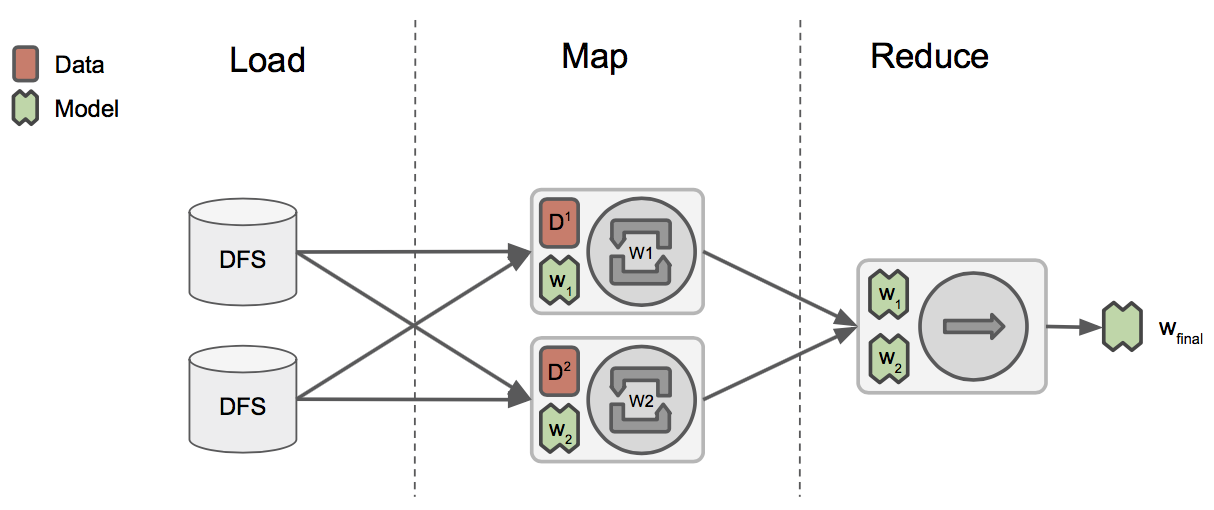
\includegraphics[width=0.9\textwidth]{img/data_parallelism.png}
\caption{Data-parallelism via MapReduce}
\label{fig:data_parallelism}
\end{figure}
In this context, data-parallelism means that $K$ machines work in parallel on the input data $D$, hence the data is distributed according to partition $\{P_k\}_{k=1}^K$ into local parts $D^k$.
Each machine maintains a local model $w_k$ that is iteratively refined based on \ref{eqn:delta_upd} until convergence, using only the local part of the input data $D^k$.
The local update is of the form
\begin{equation}
w_k^{t} = w_k^{t-1} + \Delta(w_k^{t-1},D^k)
\label{eqn:local_delta_upd}
\end{equation}
The final model $w_{final}$ is then obtained in the reduce step by averaging over all local models $w_{k}$.
\begin{equation}
w_{final} = \frac{1}{K}\sum_{k=1}^{K}w_{k}
\label{eqn:avg_sgd}
\end{equation}
Even though this approach works well in practice and gives considerable good results, it suffers from two limitations.
First, if the size of a local model $w_k$ exceeds the available memory on a single machine, the algorithm can not work properly.
This is the case e.g. for topic models at web scale or deep neural networks used in the Google Brain project \cite{dean2012large}, consisting of billions of parameters.
Second, even though the scalability improved by introducing data-parallelism the lack of parameter exchange during runtime can lead to suboptimal performance \cite{xing2015strategies} as the algorithm essentially resembles batch gradient descent, which is known to have suboptimal convergence properties compared to mini-batch or stochastic gradient descent \cite{bottou2010large} \cite{smith2016cocoa}.
In order to improve the performance, a system must be able to communicate more frequently and it must also be able to partition a model accross multiple machines to scale with the size of the model.
Following those requirements resulted in the publication of the parameter server \cite{Li2014}, which provides a framework for inter-node parallelism of iterative convergent algorithms.

\subsection{Communication}
As depicted in Figure \ref{fig:param_server}, the parameter server is a group of an arbitrary number of machines $\{S\}_{l=1}^L$, e.g. $S = \{S_1, S_2\}$ where each member of the group is responsible for storing a part of the model $\{w\}_{l=1}^L$ and making it accessible to the workers $\{W\}_{k=1}^K$, e.g. $W = \{W_1, W_2, W_3\}$, via a defined interface that is similar to a key-value store.
The model is partitioned among the machines of the server to provide optimal throughput, fault tolerance and to mitigate the effect of a model exceding the memory of a single machine.
\begin{figure}[ht]
\centering
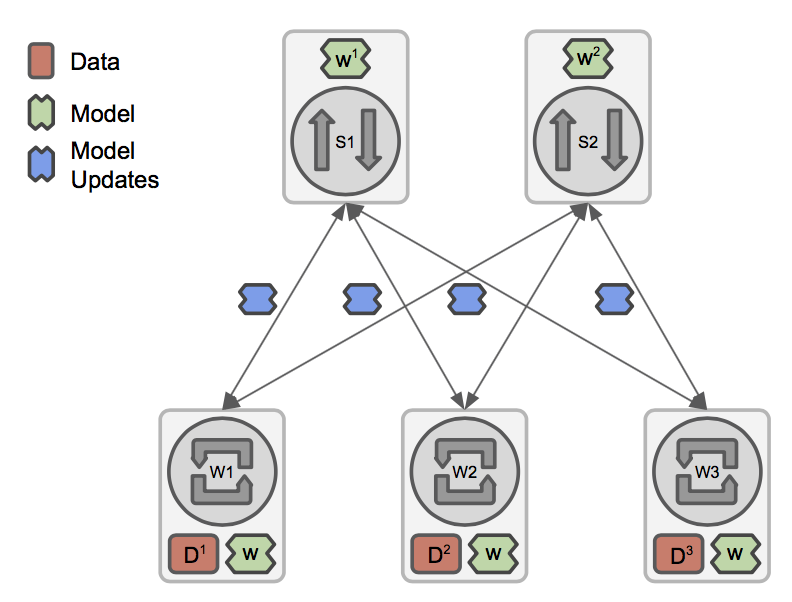
\includegraphics[width=0.7\textwidth]{img/param_server.png}
\caption{Parameter Server}
\label{fig:param_server}
\end{figure}
Each of the workers maintains a local partition of the input data $\{D\}_{k=1}^K$, which is used to iteratively compute updates for the parameters $w$ according to
\begin{equation}
\Delta w_{k_i}^{t} = \Delta(w_{k_i}^{t-1},D^k).
\label{eqn:local_delta_upd_param}
\end{equation}
In the parameter server setup, the local state $w$ acts as a cache for global parameters in order to reduce network usage.
Therefore, depending on the caching policy, $w_{k_i}$ can either be directly read either the local cache or must be retrieved from the parameter server.
Additionally to applying the update to the local model $w$, the difference $\Delta w_{k_i}^{t}$ is published to the parameter server as well, which takes care of applying it to the corresponding entry $w_i$ to make the update available to all other workers $W_i$, $i \neq k$.
In case multiple updates for the same parameter $w_i$ arive at the same time, a user defined function (UDF) needs to be provided to the server, which takes care of combining those updates so it can be applied to the parameter stored on the server.
The procedure of retrieving, updating and publishing is executed concurrently on all workers.
This enables all workers to work in parallel on the iterative parameter refinement while asynchronously updating and retrieving the parameters necessary for computing the next update.
The procedure of updating the model in parallel is also known as model-parallelism.

While this schema has been proven to work well in practice (some numbers), a couple of issues still remain when running iterative-convergent algorithms at scale using the parameter server.
According to \cite{wei2015managed} this can be viewed as finding the trade-off between algorithm throughput and data throughput.
In other words the challenge is to find a balance between the quality of parameter refinements and the quantity at which they are generated.
As with distributed systems in general, network commmunication is the bottleneck in distributed machine learning as well.
Even though due to the stochastic nature of many machine learning algorithms, the communication can be reduce compared to the exact serial algorithm, it has been proven that fresher model parameters increase the algorithm throughput per iteration \cite{langford2009slow}.
Therefore, in order to guarantee an optimal algorithm throughput, a worker should always work with the latest parameters.
On the other hand, exchanging parameter updates over the network more frequently is time consuming, which leaves less time to run local computation and therefore essentially decreases the data throughput due to increased time spent on network management.
The second issue concerns the relaxed consistency among participating workers due to reduced communication compared to the serial algorithm.
Though this is what makes the parameter server concept so powerful because it increases the data throughput by relaxing the consistency requirements when updating parameters on the server.
By decoupling the progress of workers it is possible to minimize the effect of stragglers and synchronization delay between workers \cite{ananthanarayanan2013effective}.
However, as discussed in the next section, combining model parameters obtained from workers with greatly differing algorithm progress can have a detrimental effect on algorithm throughput.
Finding the balance between algorithm throughput and data throughput can therefore be seen as consistency management.


\subsection{Consistency}
The most important part of any distributed system is the synchronization strategy used to ensure consistency among multiple machines concurrently accessing and updating some shared state.
In distributed machine learning the shared state is the model, which is for example stored in a parameter server and continously refined by updates locally computed by a worker and then published to the server.
There are three schemes used to synchronize workers during the iterative parameter refinement.
\textit{Bulk synchronous parallelization (BSP)} leads to the best algorithm throughput (convergence achieved per number of examples processed).
In this scheme, all workers are required to finish their current iteration and at the end successfully publish all updates to the parameter server.
The server then computes a refined model $w^t$ according to \ref{eqn:bsp_upd} and each worker retrieves the updated parameters before beginning the next iteration.
This synchronization scheme guarantees consistency among all nodes at all times.
\begin{equation}
w^{t} = w^{t-1} + \frac{1}{K}\sum_{k=1}^{K}\Delta(w^{t-1}_{k}, D{k})
\label{eqn:bsp_upd}
\end{equation}
While this synchronization strategy essentially recovers the sequential algorithm for a single machine and has the same convergence properties and guarantees, it suffers from a severe limitation when used in a distributed setup \cite{langford2009slow}.
In case one of the workers is for some reason a lot slower than the others the synchronization barrier imposed by BSP forces all workers to wait for this particular worker in the group.
This is well known as the straggler problem \cite{ananthanarayanan2013effective} and can seriously affect performance in a distributed environment, because the progress is limited by the slowest node in the cluster.
BSP is commonly used in MapReduce frameworks such as Hadoop and data-flow systems like Apache Spark and Apache Flink to ensure correct program execution.
The second strategy is known as \textit{total asynchronous parallelization (TAP)}.
Similar to BSP, all workers publish their locally computed parameter updates to the server after each iteration but in this case the changes are applied to the model immediately.
Therefore no waiting for other workers is required, resulting in a very high data throughput.
The straggler problem can be mitigated by this synchronization scheme as well, as depicted in Figure \ref{fig:tap_straggler}.
\begin{figure}[ht]
\centering
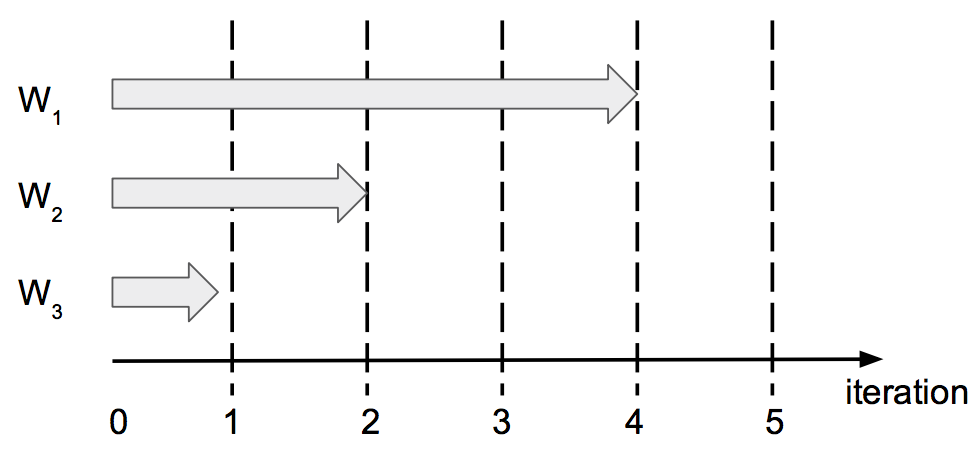
\includegraphics[width=0.6\textwidth]{img/tap_straggler.png}
\caption{Straggler in TAP}
\label{fig:tap_straggler}
\end{figure}
Even though worker $W_3$ is a straggler, which would have prevented the remaining workers $\{W_2, W_3\}$ from proceeding beyond the synchronization barrier of iteration 1, the workers can continue with their next iterations without waiting for the slower worker.
Although this consistency scheme seems to work quite well in practice \cite{Li2014}, it lacks formal convergence guarantees and can even diverge \cite{dai2014high}.
This stems from the fact that no theoretical convergence bound can be established as the divergence in iteration between workers is unbound.
\begin{figure}[ht]
\centering
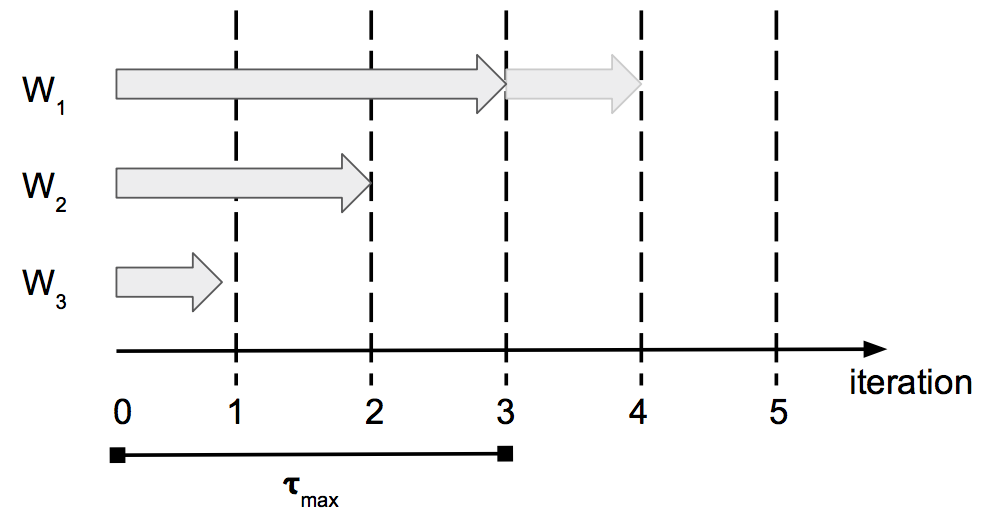
\includegraphics[width=0.6\textwidth]{img/ssp_straggler.png}
\caption{Straggler in SSP}
\label{fig:ssp_straggler}
\end{figure}
A middle ground between bulk synchronous parallelization and total asynchronous parallelization is \textit{stale synchronous parallel (SSP)} \cite{ho2013more} or \textit{bounded staleness (BS)}.
As shown in Figure \ref{fig:tap_straggler}, SSP introduces a fixed maximum delay, or staleness threshold, of $\tau_{max}$ between the slowest and fastest node.
In the example, for $\tau_{max} = 3$ worker $W_1$ is blocked and can not proceed beyond iteration 3 as the slowest worker $W_3$ has not finished its first iteration.
As soon as worker $W_3$ has completed its first iteration, $W_1$ is unblocked and can proceed as long as the difference in iteration stays below $\tau_{max}$.
SSP overcomes some of the limitations of TAP by introducing a bound on divergence in number of iterations between workers.
The staleness threshold resembles a bound which can be used to restore formal convergence guarantees while still maintaining the flexibility of asynchronous parallelization and limiting but not completely preventing the straggler problem \cite{cipar2013solving}.
In general this helps to compensate e.g. update related communication between iterations or fluctuations in worker performance, which explains why SSP works so well in practice.
